\chapter{Literature Review}

Overall methods for robot manipulation can be classified into traditional and data driven methods. Traditional methods are rule based and can be applied for structured and deterministic environments. For stochastic and unstructured environments, data driven methods are used. In this literature review, we will focus on main data driven robot manipulation methods using reinforcement learning. In reinforcement learning, training data is generated by a simulator. Reinforcement learning methods have low sample efficiency and require lot of data for training. For fast training of reinforcement learning algorithms, effective architectures like GORILLA \cite{gorila} is commonly used. In the following sections, various frameworks for efficient training of reinforcement learning algorithms and various commonly used reinforcement learning methods are discussed.

\section{SURREAL: Open-Source Reinforcement Learning Framework and Robot Manipulation Benchmark}
\begin{figure}[H]
	\centering
	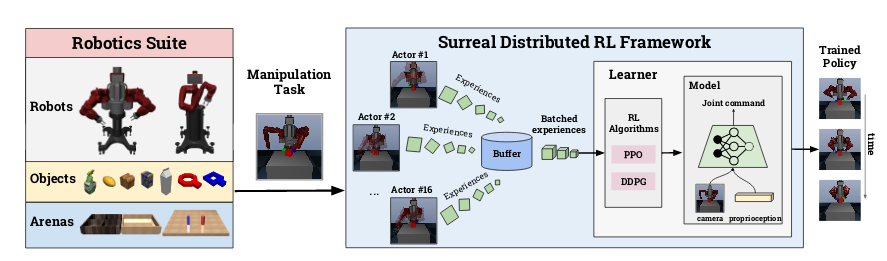
\includegraphics[scale=0.43]{surreal}
	\caption{Surreal RL framework Source: \cite{corl2018surreal}}
\end{figure}

SURREAL (Scalable Robotic Reinforcement Learning Algorithms) is an open-source framework for benchmarking reinforcement learning algorithms for different robot manipulation tasks. SURREAL framework consists of following major components

\begin{itemize}
	\item Actors - for generating training data for RL algorithms via simulation
	\item Buffer - for storing generated data from actors
	\item Learning - Core RL algorithms which updates the parameters of the model by reading data from buffer
	\item Parameter server - Storing parameters of RL models
\end{itemize}

By providing a decomposed framework, SURREAL can enable scalable reinforcement learning and can speedup RL algorithm testing by increasing computational power. SURREAL framework can be deployed on major cloud computing providers like google cloud.

SURREAL also includes a robotics suite which provides environments for common robot manipulation tasks. This enables benchmarking RL algorithm on multiple robot manipulation tasks with little effort.

\section{Reinforcement learning methods}
\begin{figure}[H]
	\centering
	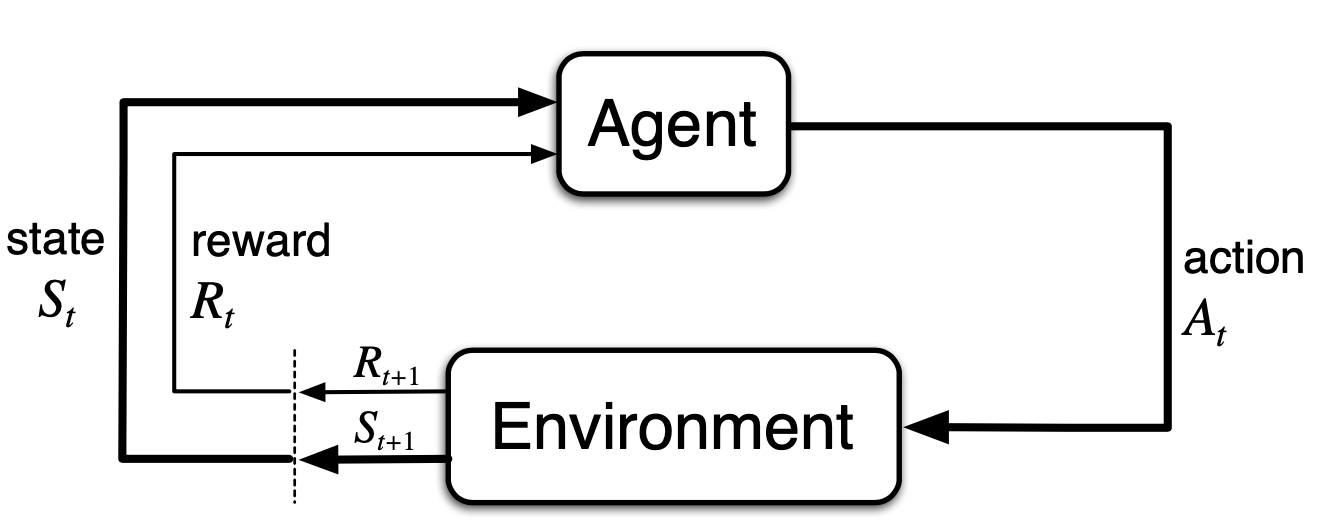
\includegraphics[scale=0.5]{mdp}
	\caption{Reinforcement Learning; Source: \cite{sutton}}
\end{figure}

In reinforcement learning, an agent learns to take actions (policy) based on measured environment state by interacting with the environment through trial and error for maximising a feedback signal (reward or value function). The main challenge in this method is requirement of large amount of data for agent to learn. Collecting large amount of data from real robot will be slow and expensive and might require manual intervention. Instead, for faster and cheaper development, agent can be trained on simulated robot manipulation environment. However policies trained on simulated environments are not directly transferable to real robots due to various differences between simulation and real environments.

\subsection{Comparing Task Simplifications to Learn Closed-Loop Object Picking}
Work done by Michel Breyer et. al. \cite{tasksimplification} found that using autoencoder to reduce dimensionality of camera data and using curriculum learning reduced the training time of agents. Also by using shaped reward functions instead of sparse reward function, they obtained 98\% success rate on simulated environment. They also found that using RANSAC for detecting and filtering surfaces from camera data while using policies trained from simulated environment on real robot gave 78\% success rate. Figure \ref{fig:tasksimplification-network} shows the network architecture used in this work.

\begin{figure}[H]
	\centering
	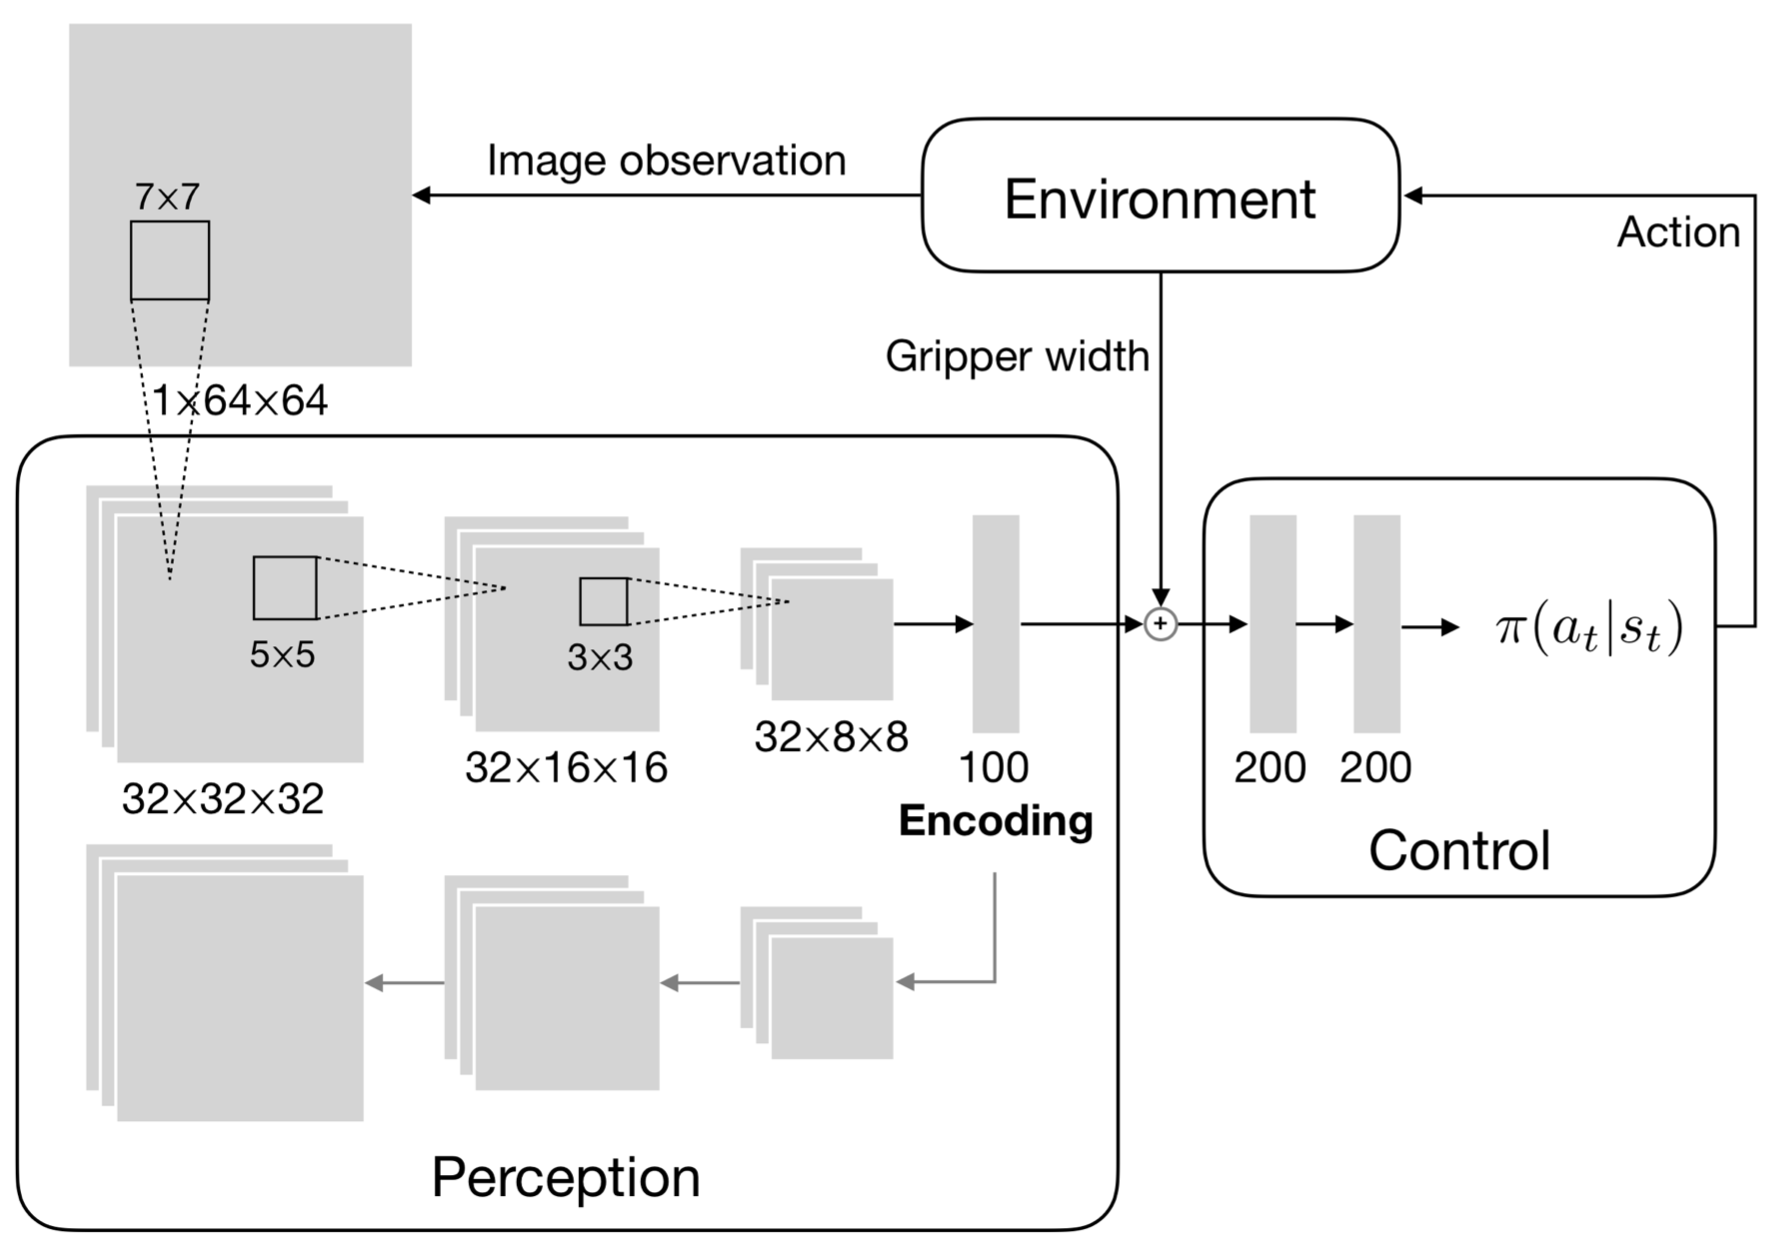
\includegraphics[scale=0.4]{task-simplification}
	\caption{Comparing Task Simplifications to Learn Closed-Loop Object Picking: Network architecture; Source: \cite{tasksimplification}}
	\label{fig:tasksimplification-network}
\end{figure}

\section{Hierarchical reinforcement learning methods}
Traditional reinforcement learning methods are data inefficient (require lot of data for training), difficult to scale (due to large action and/or state space) and brittle due to over specialisation (difficult to transfer their experience to new even similar environments) \cite{gradient}. Hierarchical reinforcement learning are intended to address these issues by learning to operate on different levels of temporal abstraction.

\subsection{Regularized Hierarchical Policies for Compositional Transfer in Robotics}
This method proposes \cite{wulfmeier2019regularized} hierarchical and modular policies for continuous control. The modular hierarchical policy used is defined as:

\begin{equation}
\pi_{\theta} (a | s, i) = \sum_{O=1}^{M} \pi_{\theta}^L(a | s, o) \pi_{\theta}^H(o | s, i)
\end{equation}

Where $\pi^H$ is the high level switching controller and $\pi^L$ is the low level sub policy. The objective is to optimize
\begin{equation}
\underset{q}{max} J(q, \pi_{ref}) = E_{i \sim I} \left[ E_{\pi, s \sim D} \left[ \sum_{t=0}^{\infty} \gamma^t r_i(s_t, a_t) | s_{t+1} \sim p(.|_t, a_t) \right] \right]
\end{equation}
subject to constraint
\begin{equation}
E_{s \sim D, i \sim I} \left[ KL(q(. | s, i) || \pi_{ref}(. | s, i)) \right] \leq \epsilon
\end{equation}

\begin{figure}[H]
	\centering
	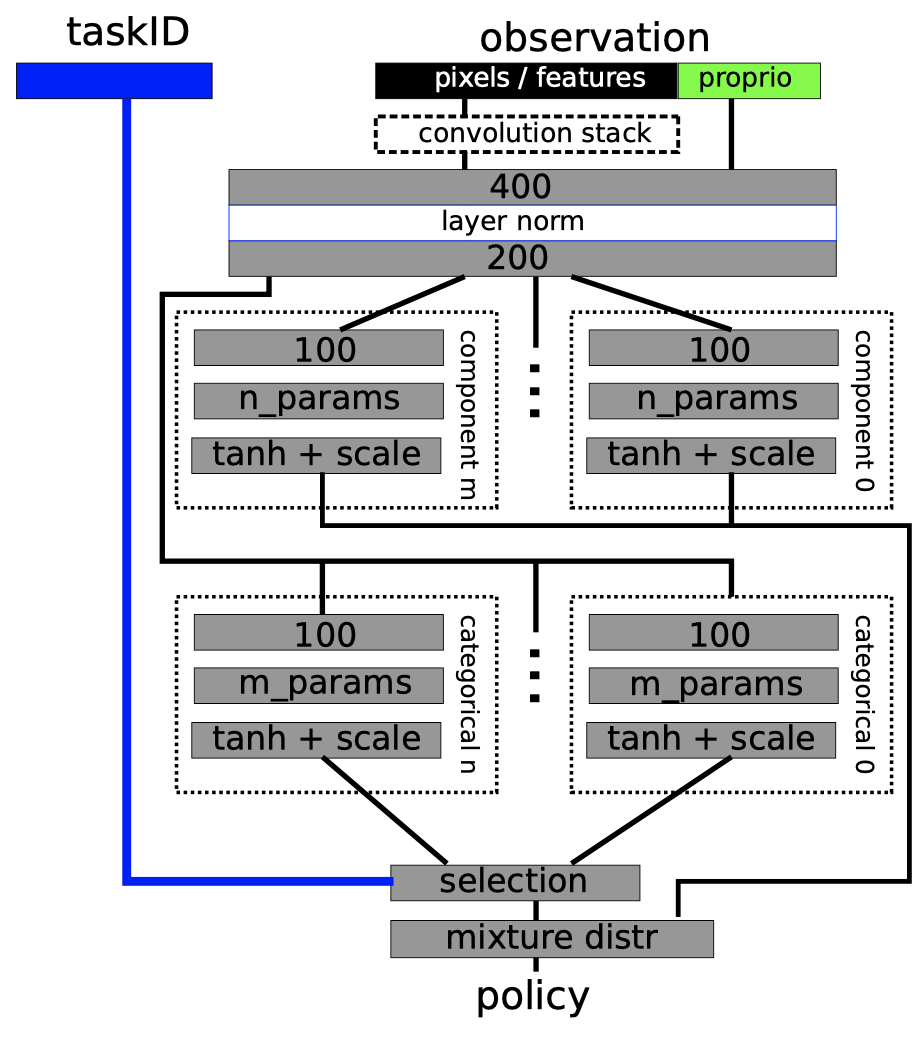
\includegraphics[scale=0.45]{rhpo-arch}
	\caption{RHPO: Network architecture}
\end{figure}

Even though SURREAL provides an efficient framework which allows scaling reinforcement learning speed with computation power and includes a good collection of prebuilt standardized environments for common robot manipulation tasks, it does not provide prebuilt support for experiment logging and tracking and it does not provide integration with RayLib, a common framework used for reinforcement learning. RayLib also includes a good collection of standard reinforcement learning algorithms and has support for both Tensorflow and PyTorch deep learning frameworks. 